% ----------------------------------------------------------
\chapter{Resultados}
% ----------------------------------------------------------
\section{Hospedagem e Pubicação}

O WebBalmy.jl foi publicado utilizando o GitHub Pages, uma ferramenta gratuita para serviços fornecidos por APIs. Ele hospeda sites estáticos criados a partir de repositórios Git, um sistema de controle de versões distribuído, usado principalmente no desenvolvimento de \textit{software}, pois salva todo o histórico de edições contido no processo de construção de um programa computacional. 

\section{Interface gráfica}

\section{Representação tridimensional}

\section{Influência de K}

\section{Diagramas de orbitais moleculares}

\section{Otimização de geometria}

\section{Índices geométricos}

\begin{figure}[htb!]
    \centering
    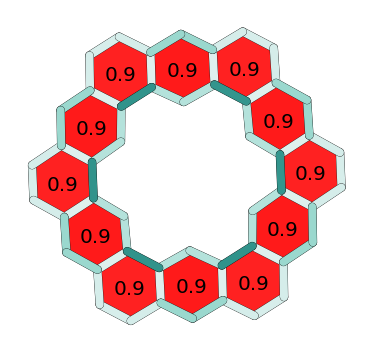
\includegraphics[width=0.36\textwidth]{images/kekulene.png}
    \caption{Caption}
    \label{fig:my_label}
\end{figure}

\begin{figure}[htb!]
    \centering
    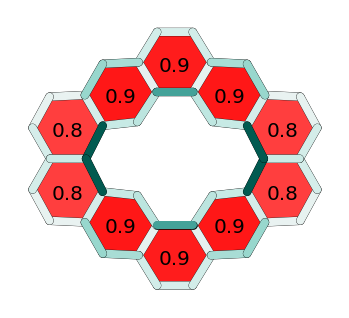
\includegraphics[width=0.36\textwidth]{images/Icosaene.png}
    \caption{Caption}
    \label{fig:my_label}
\end{figure}

\begin{figure}[htb!]
    \centering
    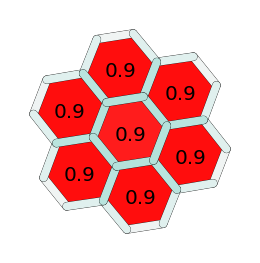
\includegraphics[width=0.28\textwidth]{images/coronene.png}
    \caption{Caption}
    \label{fig:my_label}
\end{figure}

\begin{figure}[htb!]
    \centering
    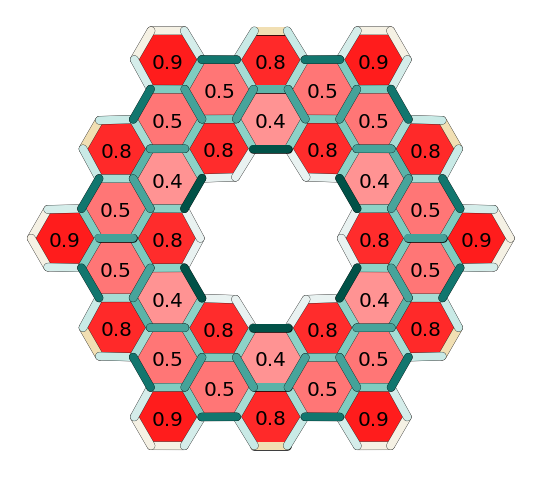
\includegraphics[width=0.6\textwidth]{images/output.png}
    \caption{Caption}
    \label{fig:my_label}
\end{figure}